\documentclass{llncs}

\usepackage[utf8]{inputenc}
\usepackage{todonotes}
\usepackage{graphicx}
\usepackage{hyperref}
\usepackage{color}
\usepackage{amsfonts}
\usepackage{amsmath}


\newcommand{\matodo}[1]{\todo[inline, color=green!50]{#1}}
\newcommand{\cetodo}[1]{\todo[inline, color=orange!50]{#1}}

\begin{document}
\title{Running experiments with confidence and sanity}
%
%\titlerunning{Abbreviated paper title}
% If the paper title is too long for the running head, you can set
% an abbreviated paper title here
%
\author{
  Martin Aumüller\inst{1}\orcidID{0000-0002-7212-6476} \and
  Matteo Ceccarello\inst{2}\orcidID{0000-0003-2783-0218}}
%
\authorrunning{M. Aumüller and M. Ceccarello}
% First names are abbreviated in the running head.
% If there are more than two authors, 'et al.' is used.
%
\institute{
  IT University of Copenhagen,
  Denmark\\
  \email{maau@itu.dk}
  \and
  Free University of Bozen, Italy\\
  \email{mceccarello@unibz.it}}
%
\maketitle              % typeset the header of the contribution
%
\begin{abstract}
Analyzing data from large experimental suites is a daily task for
anyone doing experimental algorithmics.
In this paper we report on several approaches we tried for this 
seemingly mundane task in a similarity search setting, reflecting on the many errors and consequent
mishaps.

We conclude by proposing a workflow, which can be implemented using several
tools, that allows to analyze experimental data with confidence.

\keywords{Experimental algorithmics; Experimental analysis; data analysis}
\end{abstract}

\section{Introduction}

One of the peculiar aspects of \emph{experimental algorithmics}~\cite{DBLP:conf/dimacs/Moret99}
is that the object of the study (an algorithm and its implementation)
is often crafted by the same people carrying out the analysis.
This has the advantage that the insights obtained from preliminary
investigations of early versions of an algorithm can be used to improve the
algorithm itself.
In fact, as also noted by Moret and Shapiro~\cite{DBLP:journals/jucs/MoretS01},
the understanding required for an implementation may uncover features of the
algorithms that would otherwise go unnoticed.
Furthermore, the analysis of experimental results about algorithms can give
insights about aspects that are not easily described by theoretical
models of computation~\cite{DBLP:journals/cacm/McGeoch07}.
At the same time, this feedback-based process leads to the quick
accumulation of obsolete data, referring to old versions of the
algorithms and their implementations.
Not mixing results from different versions of
an algorithm (or implementation) is an obvious requirement, which
however requires some care in practice.
In fact, oftentimes a study involves different algorithms and datasets,
each evolving at a different pace: weeks-old results might be up to date
for one algorithm, and obsolete for another.


As we shall see, the literature is mainly concerned with the design 
and analysis of
experiments, with the communication of the results,
and with reproducibility.
In this paper, instead, we report on our experience with the day to day
tasks that have to be carried out in between those three tasks, and
the approaches we developed to tackle the perils and frustrations of this 
often menial work.

\cetodo{I would like to discuss an \emph{append only} workflow, where
all past results are kept and are easily accessible, since many times
we ask ourselves "I seem to remember that once we got that result".
This is a separate issue from reproducibility, it comes before that.}
\cetodo{We might want to outline a couple of scenarios: investigating
the evolution of the results of some configuration (maybe detecting 
regressions/bugs); debugging, thus finding the change that introduced a
regression, for instance a drop in the recall or speed of the algorithm;
retrieving the most up-to date result for each configuration to do the final
analysis.}

We don't advocate for any specific technology. Rather, we propose a workflow
that can be implemented with a variety of tools that can be easily integrated
into existing setups. We demonstrate such a setup with a toy project that concerns an efficient implementation of a brute-force nearest neighbor search.

\section{Related work}

Previous works focused mainly on two areas: the design of experiments,
and reproducible research.

Moret and Shapiro~\cite{DBLP:journals/jucs/MoretS01} advocate for the
importance of complementing the theoretical analysis of algorithms
with their implementation.
McGeoch~\cite{DBLP:reference/algo/McGeoch08} gives several guidelines on how to
design and carry out experimental analyses of algorithms.
The book~\cite{DBLP:books/sp/2010BCPP} collects several contributions
on the characterization and analysis of algorithm performance.
Earlier, a Dagstuhl seminar has been devoted to the discussion of the
experimental evaluation of algorithms~\cite{DBLP:conf/dagstuhl/2000ea}.
More recently, a structured approach to the design and evaluation
of experiments has been discussed in~\cite{DBLP:series/ncs/Bartz-BeielsteinP14}.
%
Experimental studies can be influenced by contingent aspects
of the evaluation:
Bartz-Beielstein~\cite{DBLP:reference/sp/Bartz-Beielstein15} discusses
the issue of generalizing the conclusions of experimental studies.
%
McGeoch and Moret~\cite{DBLP:journals/sigact/McGeochM99} and Sanders~\cite{DBLP:conf/dagstuhl/Sanders00}
focus on the reporting of experimental results.

In recent years there has been a discussion about the lack of reproducibility
of research findings in several areas, including 
computer science~\cite{DBLP:journals/cacm/CollbergP16,Hutson725}.
Much effort has been devoted to finding a solution to this issue. Several
contributions have been collected in~\cite{stodden2014implementing} 
and~\cite{kitzes2017practice}.
Among the tools to support reproducible research, 
VisTrails~\cite{DBLP:conf/sigmod/CallahanFSSSV06} allows to
explicitly define reproducible workflows.
\texttt{knitr} and \texttt{Jupyter} take a \emph{literate programming}
approach, allowing experiment's code, analysis, and text to be interleaved
in a single "executable" document.
To solve the issues deriving from software dependencies,
some tools aim at capturing the execution
environment at runtime~\cite{DBLP:journals/cse/Guo12,davison2014sumatra,DBLP:journals/jossw/RampinCSFS16},
while others such as Docker~\cite{DBLP:journals/sigops/Boettiger15}
and Singularity~\cite{kurtzer2017singularity} follow a \emph{declarative}
approach, where the description of the execution environment is part
of the code base


\section{Challenges in running large scale experimental evaluation}
\begin{figure}[t]
  \centering
  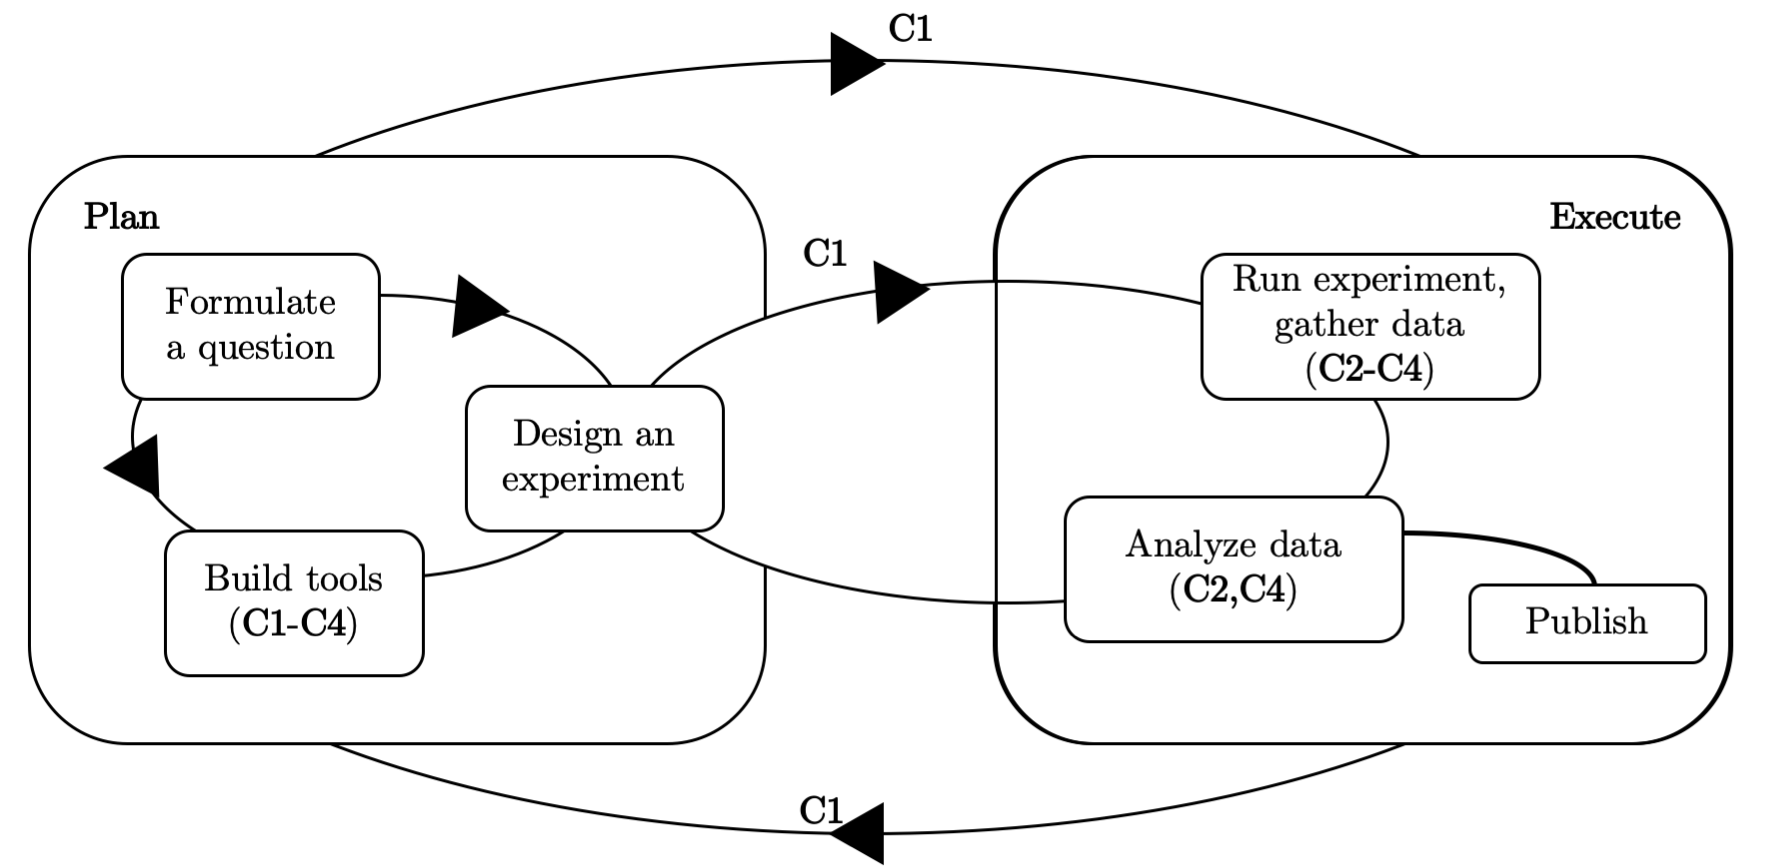
\includegraphics[width=0.8\textwidth]{figs/experiment_scheme.png}
  \caption{Overview of the different stages of an experimental challenges. Adapted from~\cite{DBLP:reference/algo/McGeoch08} by adding challenges to individual tasks and feedback loops.}
  \label{fig:overview}
\end{figure}
We define the following challenges in the  evaluation of large-scale experiments:
\begin{enumerate}
  \item[(C1)] \textbf{Feedback Loops-by-Design.} The implementations and tools support the iterative nature of an experimental study.
  \item[(C2)] \textbf{Economic Execution.} Exactly those experiments that change through code changes have to be re-run, but nothing else. 
  Moreover, only the changing parts of the experimental evaluation should be recomputed.
  \item[(C3)] \textbf{Versioning.} The ability to go back in time and compare old results to more recent ones, finding regression or bugs. This requires an \emph{append-only} workflow.
  \item[(C4)] \textbf{Machine independence.} Code and tools are designed in a way that allow them to run in a general setting.
  \item[(C5)] \textbf{Reproducibility-by-Design.} We strive for an automatic workflow that processes an experimental setup into resulting measurements used for evaluating the experiment. Results to be included into a publication should not require manual work to transform these measurements into tables and plots.
\end{enumerate}
%
We will detail these challenges in the following. 

Typically, an experimental evaluation spans several weeks, if not months. An overview of a typical experimental evaluation is given in Figure~\ref{fig:overview}. 
During this time, the experiments being run have different meanings: early
on, during the initial development, experiments are useful to find out the most
appropriate parameter ranges, find bugs, and check assumptions; later on,
experiments are devoted to the collection of the results of the study.
This is not a process that proceeds linearly from start to finish. 
Rather, the analysis of the results might prompt the modification of an algorithm
or dataset, or the introduction of new algorithms and datasets into the study,
followed by a new round of experiments.
Together with the algorithms and the datasets, also the parameterizations and the
quantities being measured are subject to evolution during the lifetime of a project (C1).

For the analysis to be sound, it is of paramount importance not to 
mix results related to different versions
of the algorithms and datasets (C3), in particular when experiments are run on a set of different machines (C4). 
The simplest solution would be to re-run the entire experimental suite whenever
something is modified. 
This usually takes a very long time, and a change might affect 
only a small part of the results, making this solution wasteful of time, energy, computational resources and money if computing resources are rented (C2). 
A potential solution might be to divide the experimental suite in smaller
components, each investigating a particular aspect, re-running only those 
affected by a change.
While this works in the short term, as the experimental study progresses
the subdivision of the experimental suite will evolve with it, leading to the
need of re-arranging the results.
On the other hand, manually re-running only parts of an experimental suite,
while reusing results from old runs, requires much care in order to exclude
obsolete results from the analysis, undermining the confidence in the soundness
of the whole analysis.
The situation worsens in the rushed final days preceding a submission:
some last minute changes are made, there is no time to re-run all the experiments,
the possibility of erroneously mixing results is very concrete. Additionally, reviewers will often demand running a new set of experiments, reporting on some other quality measures, or experimentation using different computer architectures (C2, C3, C4). \emph{Reproducibility-By-Design} (C5) requires that such wishes can be accomodated since the whole process from starting at an experimental design to a published table or figure is automated.

As for the analysis itself, it is usually executed on a machine different from the
experimental code, using a different programming language (C4).
The input of the analysis is the set of results produced by the experimental suite,
which is usually quite large due to the fact that many parameter combinations
need to be evaluated.
While the analysis code may not need the computational resourced of the 
experimental code, it still needs to execute reasonably fast, in order to be able
to examine the results interactively.
This implies that the results produced by the experiments need to be 
stored in a convenient
format that is at the same time easily manageable, convenient to transfer between
machines, and efficient to access (C2, C4).



\section{Case study: Engineering a Linear Scan}

As our toy project, we engineer a nearest neighbor search algorithm that just carries out a linear scan over the dataset. 
Formally, we are given a dataset $S \subset \mathbb{R}^d$ of $n$ points in a $d$-dimensional space with a distance measure $\text{dist}\colon \mathbb{R}^d \times \mathbb{R}^d \rightarrow \mathbb{R}$, such that given a query $q \in \mathbb{R}^d$ we want to return a point $p \in S$ that minimizes dist$(p', q)$ over all $p' \in S$.

Solving this problem via a linear scan is a straight-forward exercise in an introduction to programming class: Compare all points $p' \in S$ one by one to $q$, and keep track of the point that is closest to $q$. This results in a running time $O(nd)$ for a single query.

To make this problem more interesting (and introduce more parameters to experiment on), we consider engineering choices to speed up such a linear scan if the distance measure is the inner product $\text{dist}_{\text{IP}}(p,q) = \sum_{1 \leq i \leq d} x_i y_i$, which is analogous to cosine similarity on unit vectors. For the purpose of this project, we consider (i) input representation, (ii) parallelization, and (iii) saving distance computations as factors.

\paragraph{Input representation.}
A vector in $\mathbb{R}^d$ is traditionally represented as $d$ 64-bit floating point values (\texttt{double}). Other engineering choices are 32-bit float (\texttt{float}, or going as far as considering 16-bit representations. Since we guarantee $0 \leq x_i \leq 1$ for normalized vecors, we can use a 16-bit representations of rounded value $\lceil x_i \cdot 256 \rceil / 256$ (which could of course affect the accuracy of the result.)

\paragraph{Parallelization.}
Naïvely, the CPU has to carry out $d$ multiplications and $d-1$ additions to compute the distance of two vectors.
However, we notice that the structure is inherently parallel because the multiplications do not have data dependencies, which is ideal setup for using so-called SIMD instructions (single instruction multiple data). 
In this way, we can split up each vector into blocks of size $B$, and carry out $d/B$ parallel multiplications, $d/B$ parallel additions to aggregate terms in a register of size $B$, and one horizontal sum. 
Depending on the CPU architecture used in the experiment, $B$ is usually 128, 256, or---very recently---512 bits. Moreover, the choice of representing a single vector in $\mathbb{R}^d$ ranges gives a range of possibilities, using 32- or 64-bit floats, or use custom 16-bit representations.

\paragraph{Saving Distance Computations.} Computing the distance 
between two vectors is certainely the most expensive operation in our linear scan. Hence, if we could decide for a data point $p'$ that it probably is not the nearest neighbor looking could increase the performance of our linear scan. We include experiments with a 64-bit sketch using SimHash with probabilistic quality guarantees in our experiments. We review the approach in more detail in Appendix~\ref{app:sketches}.

\medskip

We consider this toy project representable for an experimentation task in a similarity search setting. An individual run is characterized by many different algorithms, there are feedback loops for the engeering choices, one has to handle datasets and their workloads, one has to measure certain attributes of the run, and so on. The experiment has to be carried out on different machines because of the hardware dependencies, which might mean to rent cloud instances to carry out measurements on recent hardware with $B = 512$ bit AVX512 support.

\matodo{Add discussion how challenges relate to this toy project.}

Our code is provided at \url{TODO}. For the scope of this paper, we consider the \emph{support code} that takes care of handling the setup as the main contribution.  

\section{Approaches to experimental evaluation}
We now describe a workflow we developed to address the challenges outlined
in the previous sections, demonstrating it with our case study.
We split up the discussion into different dimensions of running 
a successful experimental study. 
These dimensions are summarized in Figure~\ref{fig:discussion}. 
In the following, each dimension will be introduced with general
guidelines and a discussion of our actual solution. 

\begin{figure}
  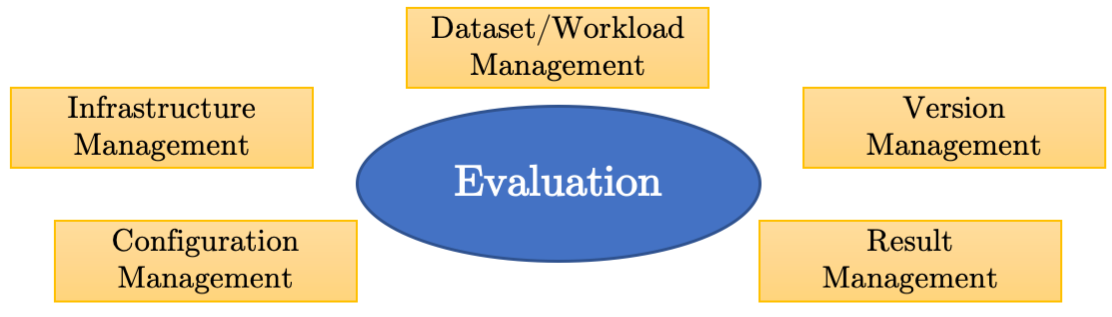
\includegraphics[width=\textwidth]{figs/discussion_points.png}
  \caption{Dimensions for running large-scale experimental evaluations.}
  \label{fig:discussion}
\end{figure}

\subsection{Manage the datasets and workloads efficiently}

\begin{itemize}
\item Dataset download and preprocessing should be automated as much as possible,
  ideally with a single script responsible to manage all the datasets.
  This makes reproducibility easier, allows to share preprocessing steps between similar datasets,
  makes it easy to relocate the experiments on a different machine, and makes all the
  decisions about datasets explicit.
  Furthermore, it enables the community to change the datasets to observe how these changes
  are reflected in the experiments.
\item Related to the above, it must be possible to create all datasets locally, 
  but the preprocessed datasets should also be shared, for instance using plain 
  \texttt{http} or a service such as \texttt{S3}.
  This makes it easier for collaborators, reviewers, and the community to re-run the
  experiments without incurring the set-up cost of the datasets.
\item Datasets should be annotated with meta-data necessary in the evaluation, 
  such as workloads and the related ground truth answers.
\item To ease debugging, a small dataset of random data that can be created in a few
  seconds should also be included.
\end{itemize}


\subsection{Manage the experimental configurations clearly}

\begin{itemize}
\item Never run experiments from the command line. Direct command line execution
  should be limited to testing.
\item Experiments should be described in one or more files. This makes it easier
  to reproduce the entire experimental suite. There are several options, which we both 
  demonstrate in the associated code:
  \begin{itemize}
    \item Files in a declarative language such as YAML listing all the combinations of
    parameters to be tested. These files are then interpreted by a script that spawns
    the appropriately configured experimental code. This approach has the advantage of
    being declarative, and the disadvantage of requiring some additional software.
    \item Shell scripts that directly invoke the experimental code using 
      the appropriate parameters. This is a more procedural approach, which however has
      the advantage of requiring very little setup.
  \end{itemize}
\item All the aforementioned experimental files should be tracked with version 
  control along with the code. Before running the experiments, any pending changes should
  be committed.
\item There should be a mechanism allowing to skip already-run configurations (see~\ref{sec:manage-results}).
  This allows both to save time (challenge XXXX) without having to continuously edit
  the configuration files to remove the configurations that don't need to be run.
\end{itemize}

\subsection{Infrastructure management}

\paragraph{The code}

Not just from the point of view of implementation, but maybe even more
prominently from the point of view of usage. That is to say:

\begin{itemize}
\item Keep parameters at the bare minimum. If a parameter never changes across
  experiments, then remove it from the tunable options. That is: keep the
  interface minimal
\item Use assertions everywhere, possibly active just during debug. This means that
  you should have a test dataset that can run in a reasonable time in debug
  mode. The problem is that often the problems arise when using large datasets
  that can be handled just in release mode.
\end{itemize}

\paragraph{Provide a Well-Defined Environment}

Your implementation will depend on many different environmental settings such as the libraries needed to run your code and the correct versions of compilers/libraries/OS that you intended to use:
\begin{itemize}
  \item Provide a containerized development environment (nowadays included in programming IDE such as \url{https://code.visualstudio.com/docs/remote/containers}.)
  \item Consider different container formats for running experiments~\cite{arango2017performance}.
  \item Use continuous integration to test all parts of the workflow
\end{itemize}

\subsection{Version everything}

Keeping the source code under version control might not be sufficient, since
source code revisions (in isolation) lack semantic meaning: you cannot tell
if a version is more recent than another without looking at the VCS DAG.
Furthermore, there are several components that may need versioning in
a project:
\begin{itemize}
  \item Algorithms implementation
  \item The schemas of the database for reporting results (or the fields of 
    the CSV files, if we don't use a database)
  \item Datasets, for which the preprocessing might evolve in time in 
    response to fixing bugs
\end{itemize}
All these components can evolve independently from one another, even within each category
(we can update just one of the many algorithms and datasets under consideration).
These changes should be recorded, but we don't want to re-run all the experiments just because
one dataset was updated. Rather, we would like to re-run only those experiments involving it.
\cetodo{This is rather similar to \texttt{make}, so we keep re-inventing the wheel, 
or the necessities are always the same.}
For this purpose, using the git version of the code is not well suited to this, as it is
shared between all the components.


\subsection{Manage the experimental results thoughtfully}
\label{sec:manage-experiments}

Some of the challenges we identified are related to the management of the results
of the experiments themselves.
Using a structured file format like CSV meets some of the requirements, like being
easy to produce and use, and easily transferrable between machines.
However, being a text-based format makes its parsing is very expensive, and
the entire dataset needs to be loaded in main memory at the beginning
of the analysis, even when we are only interested in a subset of it.\footnote{
  In our experience, when using CSV files a good part of our workday was spent 
  waiting for several gigabytes of text to be parsed into main memory.
}
Moreover, it is hard to evolve the contents of these files together with 
the project.

Our advice is to use a database to store the results, since it presents data 
conveniently indexed and removes the need for expensive parsing. Furthermore,
using database migrations~\cite{citation-needed} the database can evolve along with
the rest of the project, as demonstrated in our case study's code.
For simple projects, an embeddable database like SQLite\footnote{\url{https://sqlite.org}}
meets all the requirements: the results are stored in a single file which can be easily moved
between machines, and many languages used for the analysis (like Python and R) provide
facilities to access it.
For larger projects, where experimental code is executed on different machines, a database with
a client-server architecture\footnote{Such as PostgreSQL: \url{https://www.postgresql.org}} 
might be more suitable, as it removes the need of 
merging multiple database instances.
Using a database, furthermore, makes it very easy to detect whether 
an experiment has already been run by running an appropriate query from the experiment's code.

As the project progresses, results accumulate. To track the
\emph{provenance}~\cite{BunemanKW01} of each result, we suggest storing alongside
the parameters also the configuration file (and its version) that generated the result.

By means of database views~\cite{citation-needed} we can enforce that the analysis code
has access only to the most recent results related to each algorithm/dataset: the associated code
demonstrates how to embed a query in the database so to present only the results related to 
the most recent version of algorithms and datasets.
We stress that with this approach all the historical information of the project is preserved,
which is very important to debug the application or to reconstruct the reasons that
steered the direction of the project.

\subsection{Don't repeat yourself}

\section{Conclusions}

\bibliographystyle{alpha}
\bibliography{references}

\appendix

\section{Review: 1-bit sketches via SimHash}
\label{app:sketches}

\end{document}

